\appendix
\addcontentsline{toc}{chapter}{Annexes}
\chapter{Glossaire} \label{glossaire}

\subsubsection*{Réalité virtuelle}
Simulation informatique interactive immersive, en temps réel pouvant être visuelle, sonore ou haptique d'environnements réels ou imaginaires.

\subsubsection*{Google CardBoard}
Casque de réalité virtuelle en carton contenant des lentilles et un smartphone.

\subsubsection*{Stéréoscopique}
Technique mise en oeuvre pour reproduire une perception de 3D à partir de deux images.

\subsubsection*{Kinect version 1}
Périphérique initialement destiné à la console de jeux Xbox 360. Il permet à l'utilisateur d'interagir en utilisant son corps plutôt qu'une manette.

\subsubsection*{X3DOM}
\textsf{Framework} open source permettant d'exécuter des scènes 3D sur une page Web. Il est la composition entre \textsf{X3D} (Extensible 3D Graphics) et \textsf{DOM} (Document Object Model).

\subsubsection*{X3D}
Format de fichier graphique et multimédia orienté 3D utilisé dans \textit{X3DOM} pour l'ajout d'une scène 3D modélisée sur \textit{Blender}.

\subsubsection*{DOM} 
Standard du W3C qui décrit une interface indépendante de tout langage de programmation et de toute plate-forme, permettant à des programmes informatiques et à des scripts d'accéder ou de mettre à jour le contenu, la structure ou le style de documents HTML et XML.

\subsubsection*{NodeJS}
\textsf{Framework} logiciel et évènementiel en \textsf{JavaScript}. Il contient une bibliothèque de serveur HTTP, ce qui permet de faire tourner et de mieux contrôler un serveur Web sans avoir besoin d'un logiciel externe.

\subsubsection*{Socket.io}
\textit{Module de NodeJS} permettant d'utiliser les \textit{WebSockets}. Il permet de facilement les manipuler que ce soit du côté client ou du côté serveur.

\subsubsection*{ExpressJS}
\textit{Module de NodeJS} permettant de créer et gérer une application Web plus facilement parce qu'il s'occupe de création du serveur, il suffit donner une adresse ip et il le crée pour nous.

\subsubsection*{SocketIOC\#}
Projet disponible sur \textit{GitHub} permettant de faire communiquer un programme C\# avec un \textit{serveur NodeJS} utilisant \textit{Socket.io}.

\subsubsection*{Blender}
Logiciel de modélisation, d'animation et de rendu 3D développé par la \textsf{Fondation Blender}.

\subsubsection*{Cinema4D}
Logiciel libre de modélisation 3D de corps humains.

\subsubsection*{MakeHuman}
Logiciel de création 3D développé par \textsf{Maxon} permettant la modélisation, le texturage, l'animation et le rendu d'objets 3D.

\chapter{Cahier de bord}
Afin d'avoir un suivi durant le travail de Bachelor, un cahier de bord a été mis en place. Il était mis à jour tous les jours en notant le travail effectué, les problèmes rencontrés et des informations supplémentaires si nécessaires.
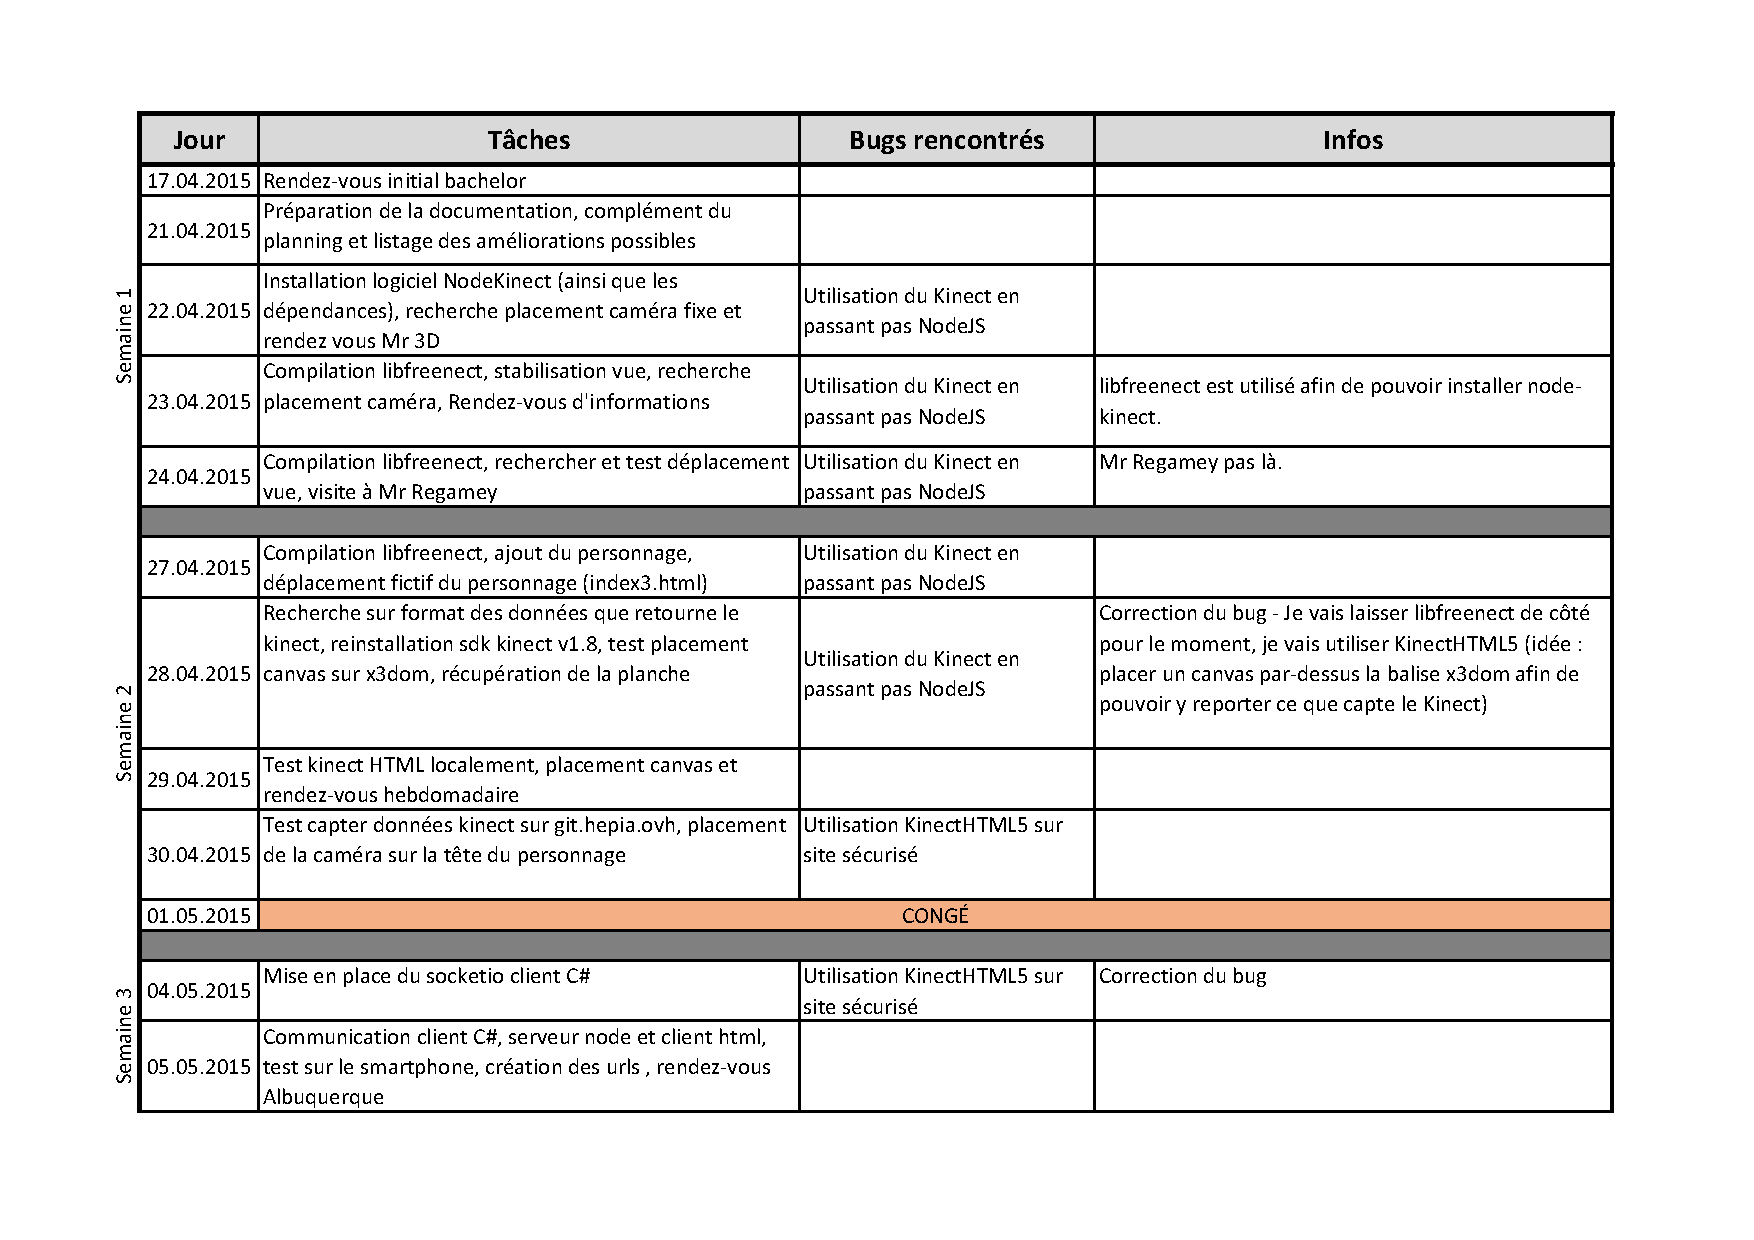
\includepdf[offset=0.8cm 0mm, pages={1,2,3,4},landscape=true, height=20cm]{../documentation/CahierBord.pdf}

\chapter{Planning} \label{plannings}
Au début du travail de Bachelor, un planning initial a été créé afin de séparer le projet \textit{Virtual-Vertigo} en tâches distinctes et d'avoir des délais à tenir. Un planning au cours du travail de Bachelor a également été créé afin de pouvoir savoir s'il y a du retard sur les tâches définies dans le planning initial.
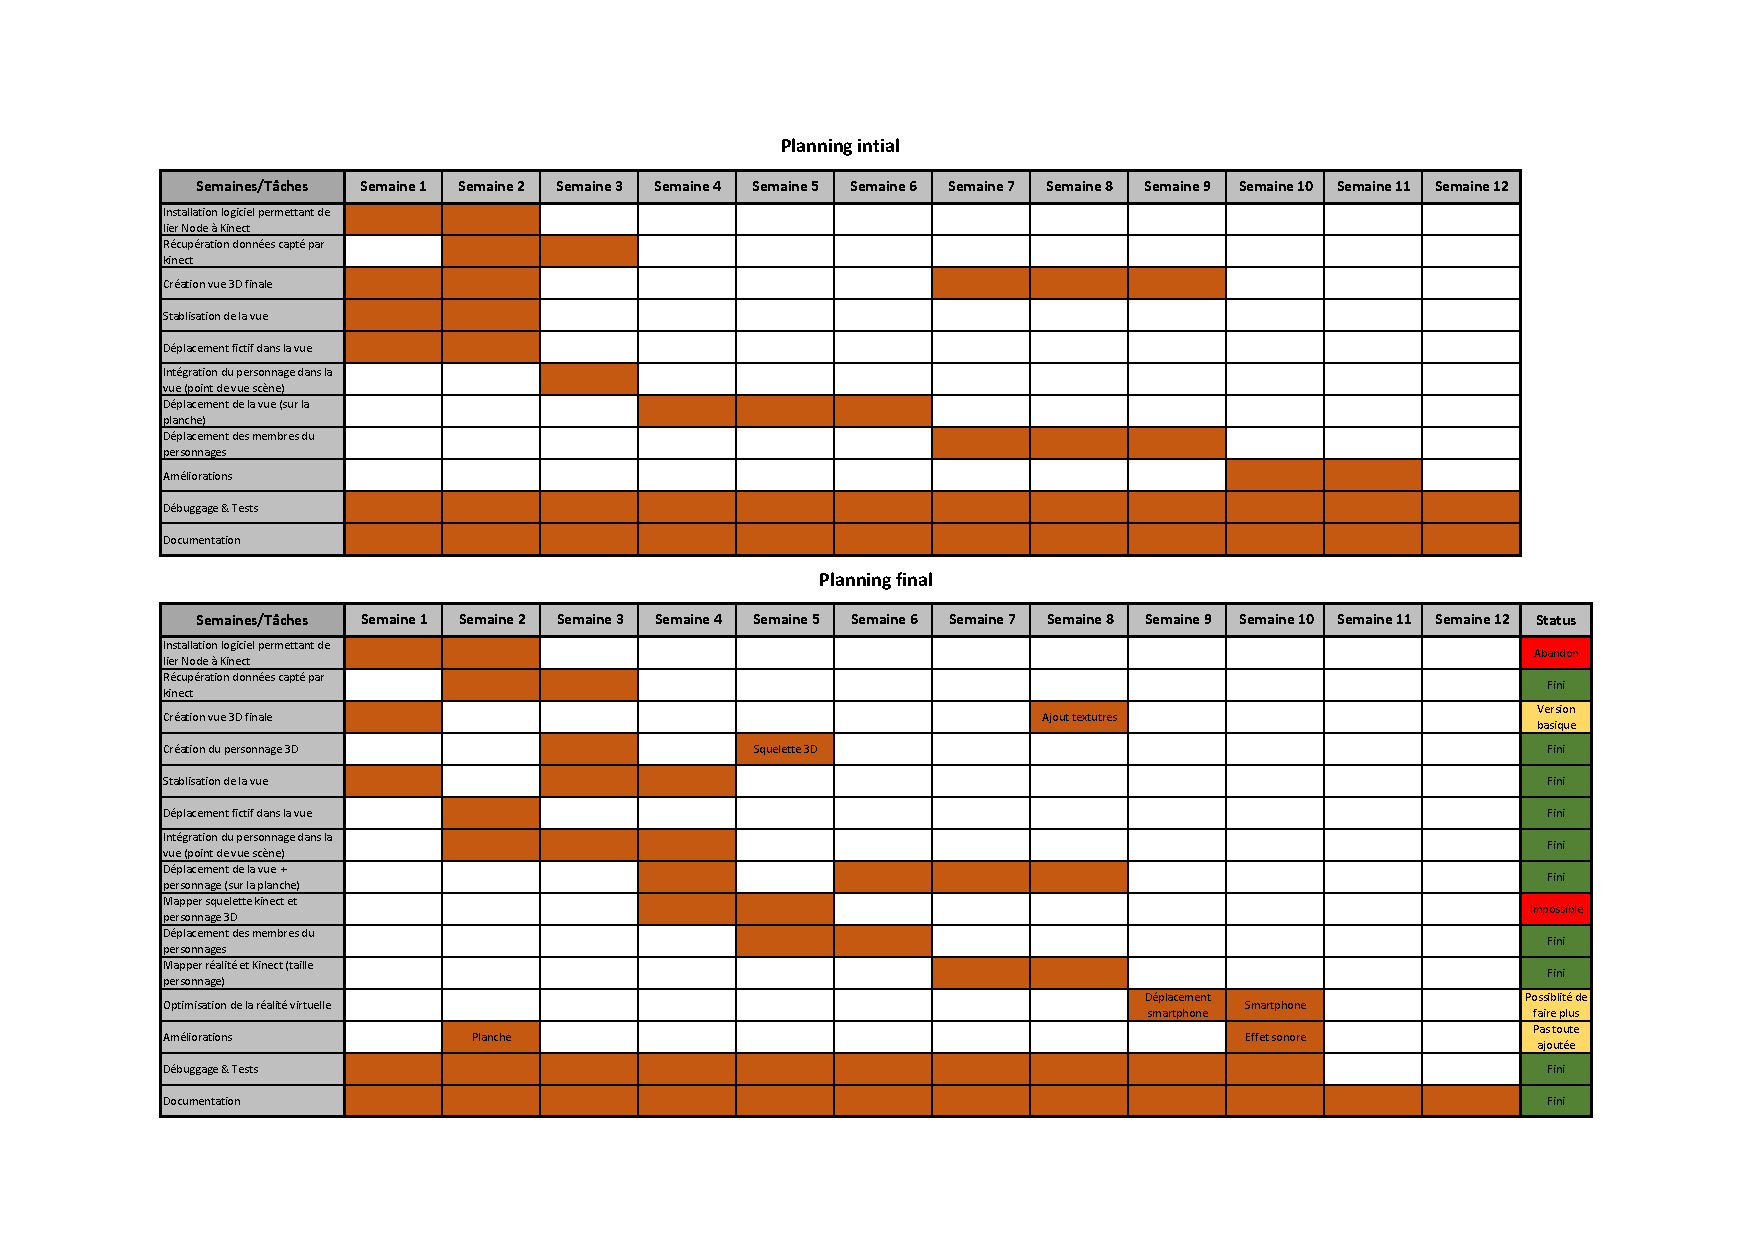
\includepdf[offset=0.8cm 0mm, pages={-},landscape=true, height=20cm]{../documentation/Planning.pdf}

\chapter{Code source}
Le code source est disponible sur un CD annexé à ce rapport. Cependant quelques extraits sont fournis ci-dessous. \\
Le fichier HTML de la scène virtuelle du \textsf{smartphone} :
 
\lstset{style=mystyle}
\begin{lstlisting}[language=Html]
<!DOCTYPE html>
<html lang="en">
  <head>
    <title>Vertigo smartphone</title>
    <meta http-equiv="Content-Type" content="text/html; charset=utf-8" />
    <link rel='stylesheet' type='text/css' href='x3dom/x3dom.css'></link>
    <script src="http://code.jquery.com/jquery-1.6.2.min.js"></script>
    <script src="/socket.io/socket.io.js"></script>
    <script src='x3dom/x3dom.js'> </script>
    <script src="./script.js"></script>
    <style>
      body { margin: 0px; overflow: hidden; }
      x3d{ width: 100%; height: 100%; }
    </style>
  </head>
  <body>
    <div onclick="fullscreen();"><h1>Fullscreen</h1></div>
    <p>Status: <label id="status">None</label></p>
    <audio id="music"  preload="auto">
    	<source src="music.mp3" type="audio/mp3">
    </audio>

    <x3d id="x3d">
      <scene id="scene">  
        <!-- define the camera and the type of naviagtion-->
        <NavigationInfo headlight="false" type='"EXAMINE"'> </NavigationInfo>
        <transform DEF='camera' id='camera' translation='-2 7 0' 
        		   rotation='0 1 0 1.57' >
        	<viewpoint id='vpp' DEF='viewpoint' position='0 0 4' 
        			   centerOfRotation='0 0 5'  orientation='1 0 0 -0.2' 
        			   fieldOfView="3.1" zNear="0.001"></viewpoint>
          	<viewpoint DEF='AOPT_CAM' position="0 0 5"  centerOfRotation="0 0 5"/>
        </transform>
  
        <!-- creation of the scene  -->
        <group id='unrendered_scene' render='false'>
          <group DEF='scene'>
            <!-- Immeuble -->
            <transform DEF='camera' id='camera' translation='0 0 0' 
            		   rotation='0 1 0 1.57'>
              <inline nameSpaceName="immeuble" mapDEFToID="true" 
              		  url="./blender/vue_semi_finale.x3d"></inline>
            </transform>

            <!-- construction du squelette du personnage -->
            <transform id='armature' translation='0 7.3 0' rotation='0 1 0 1.57' >
              <group id='armatureGroup'>
                <!-- joints -->
                <transform id='HESC'  scale='0.2 0.2 0.2' center="0 0.5 0" 
                		    translation="0 -0.5 -0.5">
                	<Inline url="./blender/membre.x3d"/>
                </transform>
                <transform id='SCSR'  scale='0.2 0.2 0.2' center="0 0.5 0" 
                		   translation="0 -0.5 -0.5">
                	<Inline url="./blender/membre.x3d"/>
                </transform>              
                <transform id='SER'   scale='0.2 0.2 0.2' center="0 0.5 0" 
                		    translation="0 -0.5 -0.5">
                	<Inline url="./blender/membre.x3d"/>
                </transform>
                <transform id='EWR'   scale='0.2 0.2 0.2' center="0 0.5 0" 
                			translation="0 -0.5 -0.5">
                	<Inline url="./blender/membre.x3d"/>
                </transform>
                <transform id='WHR'   scale='0.2 0.2 0.2' center="0 0.5 0"
                		   translation="0 -0.5 -0.5">
                	<Inline url="./blender/membre.x3d"/>
                </transform>
                <transform id='SCSL'  scale='0.2 0.2 0.2' center="0 0.5 0" 
                		   translation="0 -0.5 -0.5">
                	<Inline url="./blender/membre.x3d"/>
                </transform>             
                <transform id='SEL'   scale='0.2 0.2 0.2' center="0 0.5 0" 
                		   translation="0 -0.5 -0.5">
                	<Inline url="./blender/membre.x3d"/>
                </transform>
                <transform id='EWL'   scale='0.2 0.2 0.2' center="0 0.5 0" 
                		   translation="0 -0.5 -0.5">
                	<Inline url="./blender/membre.x3d"/>
                </transform>
                <transform id='WHL'   scale='0.2 0.2 0.2' center="0 0.5 0" 
                		   translation="0 -0.5 -0.5">
                	<Inline url="./blender/membre.x3d"/>
                </transform>
                <transform id='SCS'   scale='0.2 0.2 0.2' center="0 0.5 0" 
                		   translation="0 -0.5 -0.5">
                	<Inline url="./blender/membre.x3d"/>
                </transform>
                <transform id='SHC'   scale='0.2 0.2 0.2' center="0 0.5 0" 
                			translation="0 -0.5 -0.5">
                	<Inline url="./blender/membre.x3d"/>
                </transform>
                <transform id='HCHR'  scale='0.2 0.2 0.2' center="0 0.5 0" 
                			translation="0 -0.5 -0.5">
                	<Inline url="./blender/membre.x3d"/>
                </transform>
                <transform id='HKR'   scale='0.2 0.2 0.2' center="0 0.5 0" 
                			translation="0 -0.5 -0.5">
                	<Inline url="./blender/membre.x3d"/>
                </transform>
                <transform id='KAR'   scale='0.2 0.2 0.2' center="0 0.5 0" 
                			translation="0 -0.5 -0.5">
                	<Inline url="./blender/membre.x3d"/>
                </transform>
                <transform id='AFR'   scale='0.2 0.2 0.2' center="0 0.5 0" 
                			translation="0 -0.5 -0.5">
                	<Inline url="./blender/membre.x3d"/>
                </transform>
                <transform id='HCHL'  scale='0.2 0.2 0.2' center="0 0.5 0"
                			translation="0 -0.5 -0.5">
                	<Inline url="./blender/membre.x3d"/>
                </transform>
                <transform id='HKL'   scale='0.2 0.2 0.2' center="0 0.5 0" 
                			translation="0 -0.5 -0.5">
                	<Inline url="./blender/membre.x3d"/>
                </transform>
                <transform id='KAL'   scale='0.2 0.2 0.2' center="0 0.5 0" 
                			translation="0 -0.5 -0.5">
                	<Inline url="./blender/membre.x3d"/>
                </transform>
                <transform id='AFL'   scale='0.2 0.2 0.2' center="0 0.5 0" 
                			translation="0 -0.5 -0.5">
                	<Inline url="./blender/membre.x3d"/>
                </transform>

                <!-- members-->
                <transform id='head'><Shape>
                	<Sphere radius="0.1" /> 
                </Shape> </transform>
                <transform id='shouldercenter'><Shape>
                	<Sphere radius="0.07" />
                </Shape> </transform>
                <transform id='shoulderleft'><Shape>
                	<Sphere radius="0.07" />
                </Shape>  </transform>
                <transform id='elbowleft'><Shape>
                	<Sphere radius="0.07" />
                </Shape> </transform>
                <transform id='wristleft'><Shape>
                	<Sphere radius="0.07" />
                </Shape> </transform>
                <transform id='handleft'><Shape>
                	<Sphere radius="0.07" /> </Shape> 
               		<!-- thumb -->
                  	<transform id='thumbleft' translation="0.1 0 0">
                  	<Shape><Cylinder height="0.03" radius="0.03" /></Shape>
                  	</transform>              
                </transform>
                <transform id='shoulderright'><Shape>
                	<Sphere radius="0.07" />
                </Shape> </transform>
                <transform id='elbowright'><Shape>
                	<Sphere radius="0.07" />
                </Shape> </transform>
                <transform id='wristright'><Shape>
                	<Sphere radius="0.07" />
                </Shape> </transform>
                <transform id='handright'><Shape>
                	<Sphere radius="0.07" /> </Shape> 
                  <!-- thumb -->
                  <transform id="thumbright" translation="-0.1 0 0">
                  	<Shape><Cylinder height="0.03" radius="0.03" /></Shape>
                  </transform>   
                </transform>
                <transform id='spine'> <Shape>
                	<Sphere radius="0.07" />
                </Shape>  </transform>
                <transform id='hipcenter'><Shape>
                	<Sphere radius="0.07" />
                </Shape> </transform>
                <transform id='hipleft'><Shape>
                	<Sphere radius="0.07" />
                </Shape> </transform>
                <transform id='kneeleft'><Shape>
                	<Sphere radius="0.07" />
                </Shape> </transform>
                <transform id='ankleleft'><Shape>
                	<Sphere radius="0.07" />
                </Shape> </transform>
                <transform id='footleft'><Shape>
                	<Sphere radius="0.07" />
                </Shape> </transform>
                <transform id='hipright'><Shape>
                	<Sphere radius="0.07" />
                </Shape></transform>
                <transform id='kneeright'><Shape>
                	<Sphere radius="0.07" />
                </Shape> </transform>
                <transform id='ankleright'><Shape>
                	<Sphere radius="0.07" />
                </Shape> </transform>
                <transform id='footright'><Shape>
                	<Sphere radius="0.07" />
                </Shape> </transform>
              </group>
            </transform>
          </group>
        </group>
          
        <!-- creation of the left view -->
        <group DEF='left' render='true' class='vue'>
          <shape>
            <appearance>
              <renderedTexture id="left" stereoMode='LEFT_EYE' update='ALWAYS' 
              				  interpupillaryDistance='0.3' dimensions='800 800 4' 
              				  repeatS='false' repeatT='false'>
                <viewpoint USE='viewpoint' containerField='viewpoint'></viewpoint>
                <group USE='scene' containerField="scene"></group>
              </renderedTexture>
              <composedShader>
                <shaderPart type='VERTEX'>
                  attribute vec3 position;
                  attribute vec2 texcoord;
                  uniform mat4 modelViewProjectionMatrix;
                  varying vec2 fragTexCoord;
                  void main()
                  {
                    vec2 pos = sign(position.xy);
                    fragTexCoord = texcoord;
                    gl_Position = vec4((pos.x/2.0)-0.5, pos.y, 0.0, 1.0);
                  }
                </shaderPart>
                <shaderPart DEF="frag" type='FRAGMENT'>
                  #ifdef GL_ES
                  precision highp float;
                  #endif
                  uniform sampler2D tex;
                  uniform float leftEye;
                  varying vec2 fragTexCoord;
                  void main()
                  {
                    gl_FragColor = texture2D(tex, fragTexCoord);
                  }
                </shaderPart>
              </composedShader>
            </appearance>
            <plane solid="false"></plane>
          </shape>
        </group>
        
        <!-- creation of the right view  -->
        <group DEF='right' render='true'  class='vue'>
          <shape>
            <appearance>
              <renderedTexture id="right" stereoMode='RIGHT_EYE' update='ALWAYS' 
              				  interpupillaryDistance='0.3' dimensions='800 800 4' 
              				  repeatS='false' repeatT='false'>
                <viewpoint USE='viewpoint' containerField='viewpoint'></viewpoint>
                <group USE='scene' containerField="scene"></group>
              </renderedTexture>
              <composedShader>
                <shaderPart type='VERTEX'>
                  attribute vec3 position;
                  attribute vec2 texcoord;
                  uniform mat4 modelViewProjectionMatrix;
                  varying vec2 fragTexCoord;
                  void main()
                  {
                    vec2 pos = sign(position.xy);
                    fragTexCoord = texcoord;
                    gl_Position = vec4((pos.x + 1.0)/2.0, pos.y, 0.0, 1.0);
                  }
                </shaderPart>
                <shaderPart USE="frag" type='FRAGMENT'>
                </shaderPart>
              </composedShader>
            </appearance>
            <plane solid="false"></plane>
          </shape>
        </group>
      </scene> 
    </x3d> 
  </body>
</html>
\end{lstlisting}

La récupération des données reçues par le \textit{Kinect} en \textsf{JavaScript} :

\lstset{style=mystyle}
\begin{lstlisting}[language=JavaScript]
window.onload = function () {
	var character = $("#character");
	var vp = $("#vpp");
	var status = $("#status");
    status.text("Connecting to server...");

	 /* getting the informations of the kinect */
    // Connect to server.
    var socket = io.connect('http://'+ ip +':3000');
    status.text("Connection successful.");
   
    // Receive data FROM the server!
    socket.on("dataKinect",function(json){
        status.text("Kinect data received.");
        console.log(json);

        for (var i = 0; i < json.length; i++){
        	for (var j=0; j < jointsType.length; j++){
        		// map the joint type to his name
        		if (json[i].JointType == j)
            		position[jointsType[j].joint] =  
            		{"name" : jointsType[j].joint , 
            		"x" : json[i].Position.X.toFixed(3) * REAL, 
            		"y" : json[i].Position.Y.toFixed(3) * REAL, 
            		"z" :  json[i].Position.Z.toFixed(3)};
        	}
        }
		animate(position);
    });

 	socket.on("boneOrientation", function(boneOrientation){
 		//var startjoint = jointsType[boneOrientation.start].joint;
 		var endjoint = jointsType[boneOrientation.end].joint;

 		// rotation of the thumb 
 		if (endjoint == 'handleft')
 			$("#thumbleft").attr("rotation", 
 									boneOrientation.rotation.X.toFixed(3) + 
 									" " + boneOrientation.rotation.Y.toFixed(3) + 
 									" " + boneOrientation.rotation.Z.toFixed(3) 
 			+ " " + boneOrientation.rotation.W.toFixed(3));
 		else if (endjoint == 'handright')
 			$("#thumbright").attr("rotation", 
 									boneOrientation.rotation.X.toFixed(3) + 
 									" " + boneOrientation.rotation.Y.toFixed(3) + 
 									" " + boneOrientation.rotation.Z.toFixed(3) 
 			+ " " + boneOrientation.rotation.W.toFixed(3));
 	});
\end{lstlisting}

L'animation du personnage provenant du script \textsf{JavaScript} permettant de modifier la scène virtuelle :

\lstset{style=mystyle}
\begin{lstlisting}[language=JavaScript]
var jsonMembers = {};
var old = {};
// json with all the related members for the animation 
var relatedMembers = [
	{ "id" : "SCSL" , "A" : "shouldercenter",   "B" : "shoulderleft"},
	{ "id" : "SEL" ,  "A" : "shoulderleft",  	"B" : "elbowleft"},
	{ "id" : "EWL" ,  "A" : "elbowleft",  		"B" : "wristleft"},
	{ "id" : "WHL" ,  "A" : "wristleft",  		"B" : "handleft"},
	{ "id" : "HESC" , "A" : "head",  			"B" : "shouldercenter"},
	{ "id" : "SCSR" , "A" : "shouldercenter",   "B" : "shoulderright"},
	{ "id" : "SER" ,  "A" : "shoulderright",    "B" : "elbowright"},
	{ "id" : "EWR" ,  "A" : "elbowright",  		"B" : "wristright"},
	{ "id" : "WHR" ,  "A" : "wristright",  		"B" : "handright"},
	{ "id" : "SCS" ,  "A" : "shouldercenter",  	"B" : "spine"},
	{ "id" : "SHC" ,  "A" : "spine",  			"B" : "hipcenter"},
	{ "id" : "HCHR" , "A" : "hipcenter",  		"B" : "hipright"},
	{ "id" : "HKR" ,  "A" : "hipright",  		"B" : "kneeright"},
	{ "id" : "KAR" ,  "A" : "kneeright",  		"B" : "ankleright"},
	{ "id" : "AFR" ,  "A" : "ankleright",  		"B" : "footright"},
	{ "id" : "HCHL" , "A" : "hipcenter",  		"B" : "hipleft"},
	{ "id" : "HKL" ,  "A" : "hipleft", 			"B" : "kneeleft"},
	{ "id" : "KAL" ,  "A" : "kneeleft",  		"B" : "ankleleft"},
	{ "id" : "AFL" ,  "A" : "ankleleft",  		"B" : "footleft"} ];	
	
// animate and move the skeleton 
function animate(moyenne){

	// create the skeleton and set the data received of the kinect
   jQuery.each(position, function() {
		var name = this.name;

		$("#"+name).attr("translation",  
							position[name].x  + 
							" " + position[name].y + 
							" " +  position[name].z);
	});

	// relate the members
	for (var k=0; k<relatedMembers.length; k++)
		buildSkeleton(relatedMembers[k]);
	
	move();
}

// creation of all the skeleton
function buildSkeleton(members){
	if ((position[members.A] != undefined)&(position[members.B] != undefined)){

		// -------------------shoulder - elbow --------------------------------
		old[members.id] = {"distance" : null, "angle" : null}
		jsonMembers[members.id] = {
			"distance":calcDistance(position[members.A],position[members.B]),
			"angle":calcAngle(position[members.A],position[members.B])
		}

		positionning(members.id, position[members.A]); 
		old[members.id].distance = scaling(members.id, 
											jsonMembers[members.id].distance,
											old[members.id].distance); 
		old[members.id].angle = anime(members.id, 
										jsonMembers[members.id].angle,
										old[members.id].angle);
	}
}

// find the distance between 2 points on a cartesien plan
function calcDistance(p1, p2){
	return Math.sqrt(Math.pow((p2.x - p1.x),2) + Math.pow((p2.y - p1.y),2));
}

// find the angle between 2 points with te arctan2
// ref : http://www.w3schools.com/jsref/jsref_atan2.asp
function calcAngle(A, B){
	return -Math.atan2(B.y - A.y, A.x- B.x);
}

// put the member in his right place in the skeleton
function positionning(id, pos){
	$("#"+id).attr("translation", (pos.x) + " " +  (pos.y -0.5) + " " + pos.z);
}

// adapt the size of the membre dans rotate in fonction of the kinect
function scaling(id, distance, old){
	var distance = distance.toFixed(2);

	if (distance != old){
		$("#"+id).attr("scale", distance  +" "+ DIV_DISTANCE + " " + DIV_DISTANCE );
		old = distance;
	}

	return old;
}

// animate the members of the character
function anime(id, angle, old){
	var angle = angle.toFixed(2);
	if (angle != old){
		$("#"+id).attr("rotation", "0 0 1 " + angle);
		old = angle;
	}
	return old;
}
\end{lstlisting}


\chapter{Illustrations différence entre X3DOM et X3D}
\lstset{style=mystyle}
Comme mentionné dans le chapitre~\ref{technologies}, \textit{X3DOM} et X3D sont semblables. \\
Voici l'exemple de code \textit{X3DOM} :
\begin{lstlisting}[language=Html]
<html> 
   <head>
    <meta http-equiv="X-UA-Compatible" content="IE=edge"/> 
     <title>My first X3DOM page</title> 
     <script src='http://www.x3dom.org/download/x3dom.js'> </script> 
     <link rel='stylesheet' type='text/css' 
           href='http://www.x3dom.org/download/x3dom.css'/> 
   </head> 
   <body> 
	 <x3d width='500px' height='400px'> 
	   <scene> 
		<shape> 
		   <appearance> 
			 <material diffuseColor='1 0 0'></material> 
		   </appearance> 
		   <box></box> 
		</shape> 
		<transform translation='-3 0 0'> 
		  <shape> 
			 <appearance> 
			   <material diffuseColor='0 1 0'></material> 
			 </appearance> 
			 <cone></cone> 
		  </shape> 
		</transform> 
		<transform translation='3 0 0'> 
		  <shape> 
			 <appearance> 
			   <material diffuseColor='0 0 1'></material> 
			 </appearance> 
			 <sphere></sphere> 
		  </shape> 
		</transform> 
	   </scene> 
	</x3d> 
   </body> 
</html> 
\end{lstlisting}

Voici l'exemple d'un cylindre créé sur \textit{Blender} puis exporté au format X3D :
\begin{lstlisting}[language=Html]
<?xml version="1.0" encoding="UTF-8"?>
<!DOCTYPE X3D PUBLIC "ISO//Web3D//DTD X3D 3.0//EN" "http://www.web3d.org/specifications/x3d-3.0.dtd">
<X3D version="3.0" profile="Immersive" xmlns:xsd="http://www.w3.org/2001/XMLSchema-instance" xsd:noNamespaceSchemaLocation="http://www.web3d.org/specifications/x3d-3.0.xsd">
	<head>
		<meta name="filename" content="test.x3d" />
		<meta name="generator" content="Blender 2.72 (sub 0)" />
	</head>
	<Scene>
		<NavigationInfo headlight="true"
		                visibilityLimit="0.0"
		                type='"EXAMINE", "ANY"'
		                avatarSize="0.25, 1.75, 0.75"
		                />
		<Background DEF="WO_World"
		            groundColor="0.051 0.051 0.051"
		            skyColor="0.051 0.051 0.051"
		            />
		<Transform DEF="ShapeIndexedFaceSet_TRANSFORM"
		           translation="-0.501223 0.476330 -0.494918"
		           scale="0.488878 0.488878 0.488878"
		           rotation="0.571855 0.580078 0.580078 2.102657"
		           >
			<Transform DEF="ShapeIndexedFaceSet_ifs_TRANSFORM"
			           translation="-0.000000 0.000000 -0.000000"
			           scale="1.000000 1.000000 1.000000"
			           rotation="-0.000000 -0.000000 -0.000000 0.000000"
			           >
				<Group DEF="group_ME_ShapeIndexedFaceSet">
					<Shape>
						<IndexedFaceSet solid="true"
						                coordIndex="1 2 4 3 -1 3 4 6 5 -1 5 6 8 7 -1 7 8 10 9 -1 9 10 12 11 -1 11 12 14 13 -1 13 14 16 15 -1 15 16 18 17 -1 17 18 20 19 -1 19 20 22 21 -1 21 22 24 23 -1 23 24 26 25 -1 25 26 28 27 -1 27 28 30 29 -1 29 30 32 31 -1 31 32 34 33 -1 33 34 36 35 -1 35 36 38 37 -1 37 38 40 39 -1 39 40 42 41 -1 41 42 44 43 -1 43 44 46 45 -1 45 46 48 47 -1 47 48 50 49 -1 49 50 52 51 -1 51 52 54 53 -1 53 54 56 55 -1 55 56 58 57 -1 57 58 60 59 -1 59 60 62 61 -1 4 8 6 -1 12 10 8 -1 16 14 12 -1 20 18 16 -1 24 22 20 -1 28 26 24 -1 32 30 28 -1 36 34 32 -1 40 38 36 -1 44 42 40 -1 48 46 44 -1 52 50 48 -1 56 54 52 -1 60 58 56 -1 64 62 60 -1 4 2 64 -1 4 12 8 -1 20 16 12 -1 28 24 20 -1 36 32 28 -1 44 40 36 -1 52 48 44 -1 60 56 52 -1 4 64 60 -1 4 20 12 -1 36 28 20 -1 52 44 36 -1 4 60 52 -1 4 36 20 -1 4 52 36 -1 2 1 63 64 -1 61 62 64 63 -1 1 61 63 -1 57 59 61 -1 53 55 57 -1 49 51 53 -1 45 47 49 -1 41 43 45 -1 37 39 41 -1 33 35 37 -1 29 31 33 -1 25 27 29 -1 21 23 25 -1 17 19 21 -1 13 15 17 -1 9 11 13 -1 5 7 9 -1 1 3 5 -1 1 57 61 -1 49 53 57 -1 41 45 49 -1 33 37 41 -1 25 29 33 -1 17 21 25 -1 9 13 17 -1 1 5 9 -1 1 49 57 -1 33 41 49 -1 17 25 33 -1 1 9 17 -1 1 33 49 -1 1 17 33 -1 "
						                >
							<Coordinate DEF="coords_ME_ShapeIndexedFaceSet"
							            point="0.000000 0.000000 0.000000 0.000000 1.000000 -1.000000 0.000000 1.000000 1.000000 0.195090 0.980785 -1.000000 0.195090 0.980785 1.000000 0.382683 0.923880 -1.000000 0.382683 0.923880 1.000000 0.555570 0.831470 -1.000000 0.555570 0.831470 1.000000 0.707107 0.707107 -1.000000 0.707107 0.707107 1.000000 0.831470 0.555570 -1.000000 0.831470 0.555570 1.000000 0.923880 0.382683 -1.000000 0.923880 0.382683 1.000000 0.980785 0.195090 -1.000000 0.980785 0.195090 1.000000 1.000000 0.000000 -1.000000 1.000000 0.000000 1.000000 0.980785 -0.195090 -1.000000 0.980785 -0.195090 1.000000 0.923880 -0.382683 -1.000000 0.923880 -0.382683 1.000000 0.831470 -0.555570 -1.000000 0.831470 -0.555570 1.000000 0.707107 -0.707107 -1.000000 0.707107 -0.707107 1.000000 0.555570 -0.831470 -1.000000 0.555570 -0.831470 1.000000 0.382683 -0.923880 -1.000000 0.382683 -0.923880 1.000000 0.195090 -0.980785 -1.000000 0.195090 -0.980785 1.000000 -0.000000 -1.000000 -1.000000 -0.000000 -1.000000 1.000000 -0.195091 -0.980785 -1.000000 -0.195091 -0.980785 1.000000 -0.382684 -0.923879 -1.000000 -0.382684 -0.923879 1.000000 -0.555571 -0.831469 -1.000000 -0.555571 -0.831469 1.000000 -0.707107 -0.707106 -1.000000 -0.707107 -0.707106 1.000000 -0.831470 -0.555570 -1.000000 -0.831470 -0.555570 1.000000 -0.923880 -0.382683 -1.000000 -0.923880 -0.382683 1.000000 -0.980785 -0.195089 -1.000000 -0.980785 -0.195089 1.000000 -1.000000 0.000001 -1.000000 -1.000000 0.000001 1.000000 -0.980785 0.195091 -1.000000 -0.980785 0.195091 1.000000 -0.923879 0.382684 -1.000000 -0.923879 0.382684 1.000000 -0.831469 0.555571 -1.000000 -0.831469 0.555571 1.000000 -0.707106 0.707108 -1.000000 -0.707106 0.707108 1.000000 -0.555569 0.831470 -1.000000 -0.555569 0.831470 1.000000 -0.382682 0.923880 -1.000000 -0.382682 0.923880 1.000000 -0.195089 0.980786 -1.000000 -0.195089 0.980786 1.000000 "
							            />
						</IndexedFaceSet>
					</Shape>
				</Group>
			</Transform>
		</Transform>
	</Scene>
</X3D>
\end{lstlisting}

\chapter{Fichiers X3DOM}
Le fichier x3dom.js étant illisible il ne vous sera pas transmis cependant voici le fichier x3dom.css permettant d'afficher de la réalité virtuelle sur le Web :
\begin{lstlisting}[language=Html]
/*
 * X3DOM JavaScript Library
 * http://www.x3dom.org
 *
 * (C)2009 Fraunhofer IGD, Darmstadt, Germany
 * Dual licensed under the MIT and GPL
 *
 * Based on code originally provided by
 * Philip Taylor: http://philip.html5.org
 */

body {
  background-color: white;
  font-family: Helvetica, sans-serif;
  font-size: 12px;
}

X3D, x3d {
  position:relative;    /* in order to be able to position stat-div within X3D */
  float:left;           /* float the element so it has the same size like the canvas */
  cursor:pointer;
  margin: 0;
  padding: 0;
  border: 1px solid #000;
}

object {
  margin: 0;
  padding: 0;
  border: none;
  z-index: 0;
  width:100%;
  height:100%;
  float:left;
}

X3D:hover, 
x3d:hover, 
.x3dom-canvas:hover {
  -webkit-user-select: none;
  -webkit-touch-callout: none;
}

.x3dom-canvas {
  border:none;
  cursor:pointer;
  cursor:-webkit-grab;
  cursor:grab;
  width:100%;
  height:100%;
  float:left;
}

.x3dom-canvas-mousedown {
  cursor:-webkit-grabbing;
  cursor:grabbing;
}

.x3dom-canvas:focus {
    outline:none; 
}
.x3dom-progress {
    margin: 0;
    padding: 6px 8px 0px 26px;
    left: 0px;
    top: 0px;
    position: absolute;
    color: #0f0;
    font-family: Helvetica, sans-serif;
    line-height:10px;
    font-size: 10px;
    min-width: 45px;
    min-height: 20px;
    border: 0px;
    background-position: 4px 4px;
    background-repeat: no-repeat;
    background-color: #333;
    background-color: rgba(51, 51, 51, 0.9);
    z-index: 100;
    background-image: url('data:image/gif;[...]);
}

.x3dom-progress.bar span {
  position: absolute;
  left: 0;
  top: 0;
  line-height: 20px;
  background-color: red;
}


.x3dom-statdiv {
    margin: 0;
    padding: 0;
    right: 10px;
    top: 10px;
    position: absolute;
    color: #0f0;
    font-family: Helvetica, sans-serif;
    line-height:10px;
    font-size: 10px;
    width: 75px;
    height: 70px;
    border: 0px;
}

#x3dom-state-canvas {
    margin: 2px;
    padding: 0;
    right: 0%;
    top: 0%;
    position: absolute;
}

#x3dom-state-viewer {
  position: absolute;
  margin: 2px;
  padding: 5px;
  width: 135px;
  top: 0%;
  right: 0%;
  opacity: 0.9;
  background-color: #323232;
  z-index: 1000;
  font-family: Arial, sans-serif;
  color: #C8C8C8;
  font-weight: bold;
  text-transform: uppercase;
  cursor: help;
}

.x3dom-states-head {
  display: block;
  font-size: 26px;
}

.x3dom-states-head2 {
  font-size: 10px;
}

.x3dom-states-list {
  float: left;
  width: 100%;
  border-top: 1px solid #C8C8C8;
  list-style: none;
  font-size: 9px;
  line-height: 16px;
  margin:0;
  padding: 0;
  padding-top: 2px;
}

.x3dom-states-item  {
  width: 100%;
  float: left;
}

.x3dom-states-item-title {
  float: left;
  margin-left: 2px;
}

.x3dom-states-item-value {
  float: right;
  margin-right: 2px;
}

.x3dom-touch-marker {
	display: inline;
    padding: 5px;
	border-radius: 10px;
    position: absolute;
    font-family: Helvetica, sans-serif;
    line-height:10px;
    font-size: 10px;
    color: darkorange;
    background: cornsilk;
    opacity: 0.6;
    border: 2px solid orange;
	z-index: 200;
}

.x3dom-logContainer {
    border: 2px solid olivedrab;
    height: 200px;
    padding: 4px;
    overflow: auto;
    white-space: pre-wrap;
    font-family: sans-serif;
    font-size: x-small;
    color: #00ff00;
    background-color: black;
    margin-right: 10px;
}

.x3dom-nox3d {
    font-family: Helvetica, sans-serif;
    font-size: 14px;
    background-color: #eb7a7a;
    padding: 1em;
    opacity: 0.75;
}

.x3dom-nox3d p { 
    color: #fff;
    font-size: 14px;
}

.x3dom-nox3d a { 
    color: #fff;
    font-size: 14px;
}


/* self-clearing floats */
.group:after {
  content: "."; 
  display: block; 
  height: 0; 
  clear: both; 
  visibility: hidden;
}
\end{lstlisting}

\chapter{Tutoriel d'installation des outils et utilisation du projet Virtual-Vertigo}

Afin de vous permettre d'installer et d'utiliser le projet \textit{Virtual-Vertigo}, ci-dessous, un tutoriel d'installation et manuel utilisateur.
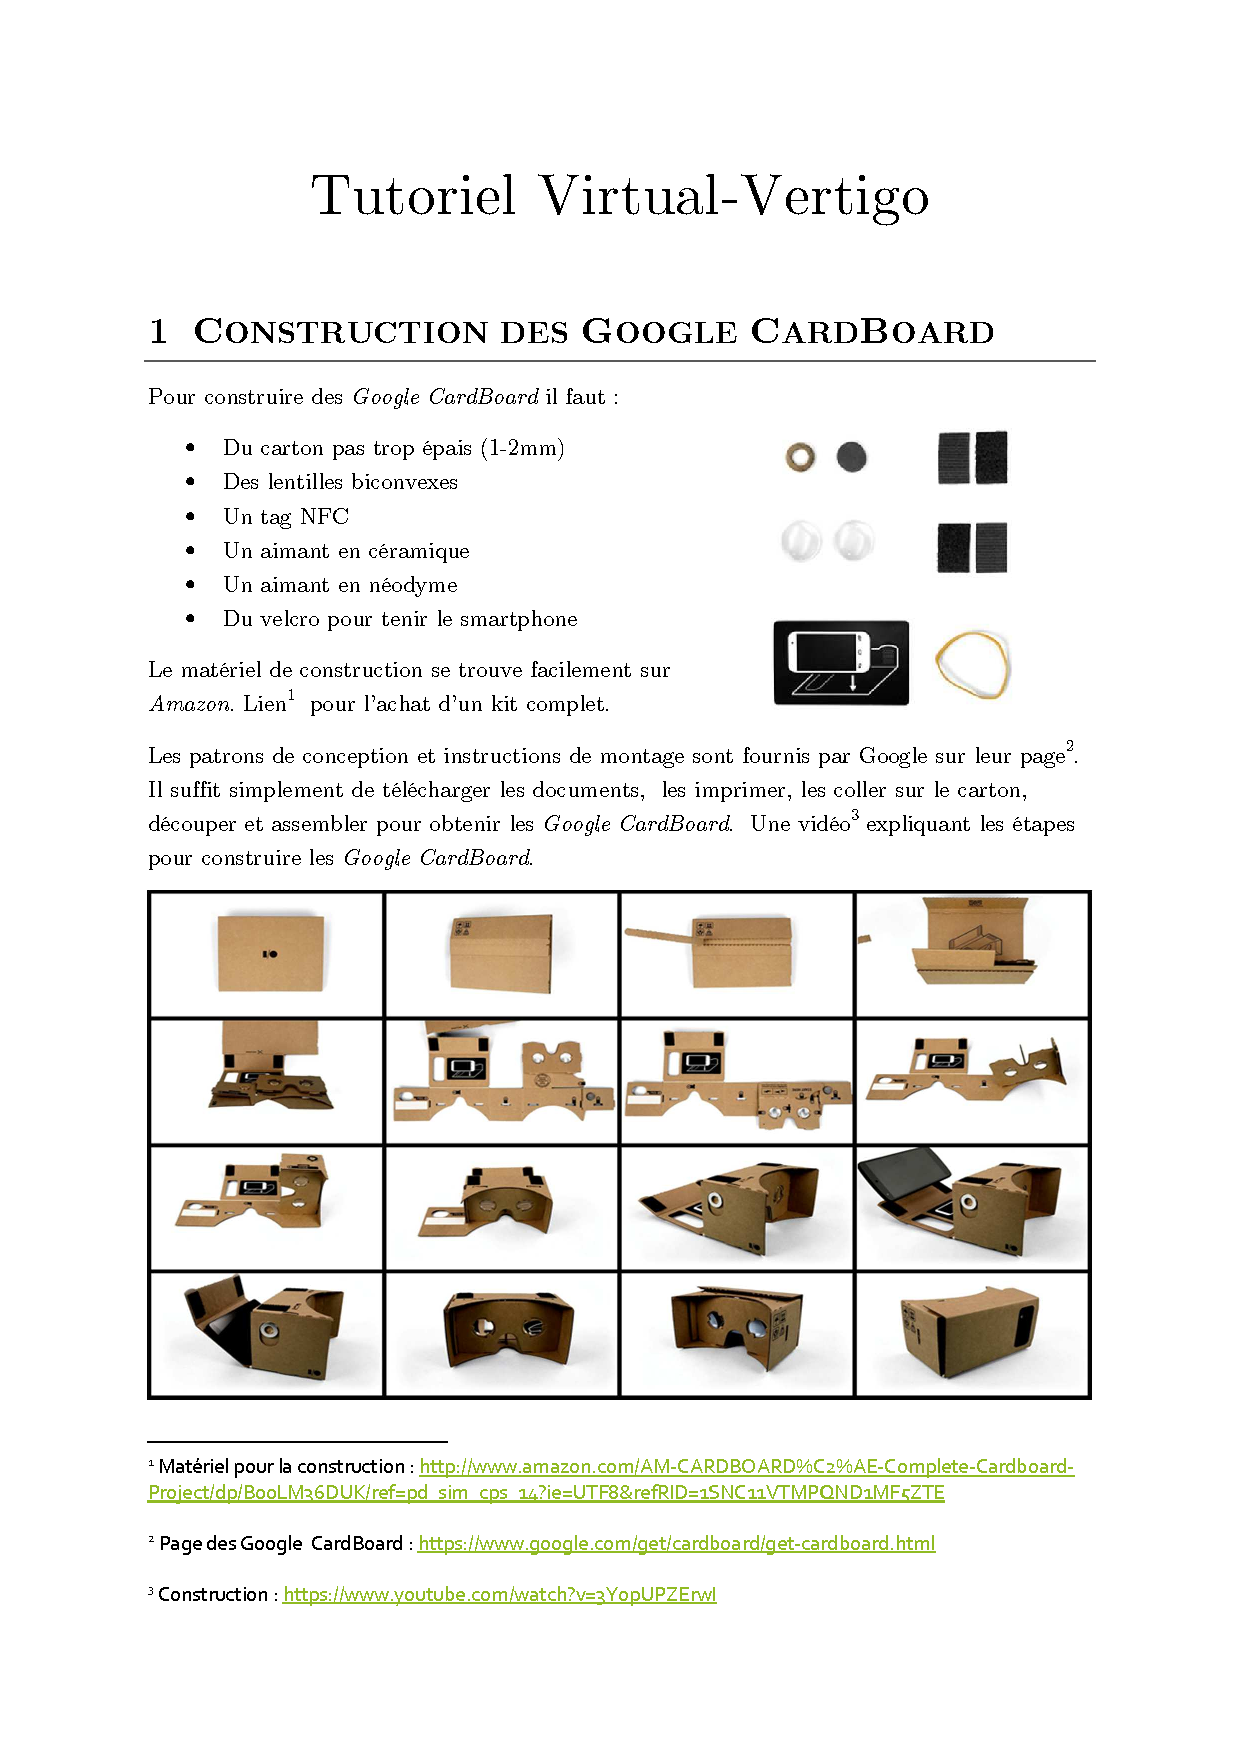
\includepdf[offset=0.8cm 0mm, pages={-}, width=20cm]{../documentation/Tutoriel.pdf}



 
